% put environments that should be ignored by texcount here, e.g., here lstlisting for code

%TC:envir lstlisting [] ignore

%for reference to this section
\section{Introduction}
\label{section:Introduction}

This paper aims to get a correlation between pedestrian traffic and route satisfaction. Given an open GPS Trajectories Dataset from the OpenStreetMap project, the research was conducted on the historical walking data in the City of Salzburg in Austria. Due to the city's historical growth, footpaths, pedestrian areas, and private and public transport roads are limited to change and urban development (SOURCE). 

\autocite[]{Netsch2021}

Historical traffic pattern mining and analysis for traffic forecasting and improving traffic flow is nothing new to vehicle traffic management. Multiple studies focus on collecting data, analyzing patterns, and forecasting traffic flow for vehicle traffic. 

Is it possible to increase satisfaction by recommending alternative, less populated routes to tourist attractions using pedestrian path model techniques?

The research is going to be structured into a background section, related work, a section describing the methods used, a system overview, implementation details and an evaluation section.

\section{Background}
Walking and choosing routes in the city of Salzburg is due to the big tourism never a simple task. Many shortest routes are going through points of interests and showplaces used by tourist agencies for their route planning making the daily commuting hard for locals. The cities street network due to its historical growth also has not the biggest number of alternative routes for walking to offer. That results in packed walking paths during the entire year.

Further, the covid pandemic has brought a factor of distancing and trying to avoid big crowds 


Lorem ipsum dolor sit amet, consectetur adipiscing elit. 

\section{Related Work}
Introduce why this specific related work is important for your own work. Which areas do you cover and why? What do you take as inspiration and what do you do differently/improve upon? 

\autocite[]{Sevtsuk2021}

\autocite[]{Delling2012}
\autocite[]{Hashemi2017}
\autocite[]{Qiu2015}
\autocite[]{Hendawi2019}
\autocite[]{Huber2016}

\autocite[]{Zhang2012}

\section{Method}

Proposing the alternative route will be done by using the influence of historical pedestrian traffic to calculate a route with fewer interactions for the traveler to get to the same goal. This will be done by analyzing historical GPS trajectories and using a customized routing engine to propose a route then evaluated through a trail run. 

To be able to use those historical pedestrian travel patterns a new route a map, map data, mapping tools and a route engine needed to be found and selected according to the researches terms. For that an in depth research of services and solutions was carried out using keywords like "Mapping", "placeholder" using online search engines.

Outcome of that research were solutions both commercially and open-source.

Commercial applications and tools like Google Maps \footnote{\url{https://developers.google.com/maps}}, Mapbox \footnote{\url{https://www.mapbox.com/}} or Here \footnote{\url{https://developer.here.com/}} offer a lot of services to conduct operations on their provided map instances yet the free quotas and the customization for the mapping tools and routing are very limited. 

Due to that limitation of customization, which was one of the main terms for the method and tools selection open-source alternatives that enable an adaption had to be taken in consideration. And the biggest and most popular open-source project, the OpenStreetMap (OSM) \footnote{\url{https://www.openstreetmap.org/}} and its ecosystem of mapping tools, routing engines and community fit ideally to be used further. 

Given crowdedness as the main factor in calculating a new route, the crowdedness has to be measured to add traffic as a parameter to that route calculation. This will be achieved creating historical traffic patterns. To create such historical pedestrian traffic/walking patterns, a solid Data-set is needed so the routing engine can be configured to be adapted to the influence of the walking patterns. 

% To be able to propose a new route a map, map data, mapping tools and a route engine needed to be selected. 

% Commercial applications and tools like Google Maps, Mapbox or Placeholder offer a lot of services to conduct operations on their maps yet the customization for the mapping tools and routing are very limited. 

% Therefore open-source alternatives that allow and enable adaptions had to be taken in consideration. And the biggest and most popular open-source project, the OpenStreetMap (OSM) project and its ecosystem of mapping tools, routing engines and community 

% As the main factor of the research is the crowdedness of given pedestrian routes
% a way of measuring and adding traffic as a parameter to calculate new routes 
% an alternative route proposal a way of proposing that alternative is needed. The main factor traffic


To create the historical pedestrian traffic/walking patterns, a solid Data-set is needed so the routing engine can be configured to be adapted to the influence of the walking patterns. 

Searching for a Data-set that is viable for further analysis was not an easy task. There is no publicly available data from the city itself. Also, local research institutions contacted during the research period have no such data available. Therefore the OSM (OpenStreetMap) Project and its Database of public traces came in handy. Their collection is publicly accessible to be extracted, verified, classified, and then used to create a historical pedestrian traffic pattern for the part of the city that was used to create the alternative route.

% \subsection{Map / Map Data}

\subsection{OpenStreetMap}

The OpenStreetMap is a free, editable map of the whole world that is being built by volunteers largely from scratch and released with an open-content license. 
\autocite[]{wiki:about}

The project was established in 2004 and has since become the Internet's most well-known example of Volunteered Geographic Information (VGI). \autocite[]{JokarArsanjani2015} 

The OSM mission statement came out of this simple concept, which was to produce a free, editable map of the world through collaboration. Instead of focusing on outputs in the form of cartographic products and maps, OSM's core is a geographical database including geographic data and information from around the world. \autocite[]{Antoniou2017}

Number of users	8805780
Number of uploaded GPS points	11771986020
Number of nodes	7835601984
Number of ways	877995015
Number of relations	10104639


\subsection{OpenStreetMap Data}

To work with the OpenStreetMap Project, the underlying structure has to be analyzed to understand its principles. As a Geo-data provider, OSM describes all physical, natural, and human-made objects in a landscape that can be mapped as features. To represent the features, OSM uses Elements attached with Tags. Elements are the basic components of its conceptual data model of the physical world.    

There are three types of elements:

\begin{enumerate}
    \item Nodes
    
    A node is a point on the earth's surface that is identified by its latitude and longitude. Each node includes a unique identifier and a pair of coordinates. 
    
    \item Ways
    
    A way is an ordered list of two to two thousand nodes that defines a polyline. Typically, a way is a linear land feature (such as a road, wall, or river).
    
    \item Relations
    
    A relation is a multi-purpose data structure that documents a relationship between two or more data elements (nodes, ways, and/or other relations).
    
\end{enumerate}

Each of the aforementioned items can have one or more associated tags. Tags are key and value pairs which describe the meaning of a particular element. 

Therefore, the key describes a subject, category, or type of feature.
Keys can be qualified with prefixes, infixes, or suffixes to form super- or sub-categories, as well as namespace. For name keys, common namespaces include a language specification and a date namespace specification.

The value provides information about the feature specified by the key.
Typically, values consist of free-form text, one of a set of distinct values, multiple values from an enumeration, or a numeric value, such as a distance.
The tag's value is required, even if the key is self-explanatory. 


% OSM is principally a collection of geodata, meaning it is not the map itself but more the information on top of a visual map, 

% As OSM is a collection of map data 

% Elements are the basic components of OpenStreetMap's conceptual data model of the physical world. Elements are of three types:

%     nodes (defining points in space),
%     ways (defining linear features and area boundaries), and
%     relations (which are sometimes used to explain how other elements work together).



\subsection{OpenStreetMap Editing API}

The OSM Editing API is a collection of APIs based on RESTful API principles. There are API calls to create, read, update, and delete the three fundamental elements that makeup OpenStreetMap's map data. They each return or expect the data for the elements in an XML format.
\autocite[]{wiki:api}

% \subsection{Map Tools}

\subsection{Java OpenStreetMap Editor}

OSM is an openly accessible spatial database which any contributor can supply geodata to and whose existing data any contributor can also edit. It is therefore very important that software tools be available to support this editing work for contributors. The OSM wiki contains an extensive list of OSM data editing tools56
and a comparison of their characteristics. In this section we outline five of the most famous and well known OSM editors

The Java OpenStreetMap Editor (JOSM) \footnote{\url{https://josm.openstreetmap.de/}} is an an extensible Java editor for OSM and is considered an editor for skilled OSM contributors. 

It ‘supports loading GPX tracks, background imagery and OSM data from local sources as well as from online sources and allows’ direct editing of the OSM data; a number of plugins provide other advanced functions. 

JOSM is an extensible editor for ​OpenStreetMap (OSM) for ​Java 8+.

 It supports loading GPX tracks, background imagery, and OSM data from local sources as well as from online sources and allows to edit the OSM data (nodes, ways, and relations) and their metadata tags. 
 
 


% \subsection{Routing Engine}


\subsection{Open Source Routing Machine}

The Open Source Routing Machine (OSRM) \footnote{\url{http://project-osrm.org/}} is an open-source routeing engine intended for use with OpenStreetMap data. OSRM calculates the shortest path using contraction hierarchies or multilevel Dijkstra's rather than an A* variation, unlike the majority of routing servers. \autocite[]{Delling2012}

In addition to chronological routing, OSRM also enables map matching, traveling salesman issue resolution, and the generation of vector tiles with routing metadata. Both the routing and the map matching services come in handy and will be used to propose the alternative route. 

\subsubsection{Route service}

Determines the quickest route between the specified points. 

To describe the routing behavior of various transport modes, such as automobile, bicycle, and foot OSRM uses profiles. A profile defines whether it is possible to route down a particular type of path, whether it is possible to pass a specific node, and how quickly we will move when we do. This effects the creation of the routing graph and, consequently, the output routes. Further, as there are multiple ways to determine the optimal path, when calculating a route from A to B, there is a need for distinct profiles. Due to the fact that speeds vary on various types of roadways, the shortest route and the fastest route are often distinct. But there are plenty additional alternatives. A user may choose a route that passes through parks or other green areas, even if the length and distance are slightly longer. 

To address this, OSRM does not merely select the fastest routes. Instead, it employs the concepts of weight and rate. The rate is an abstract measurement that can be assigned to any method to make certain methods desirable to others. The routing algorithm will favor high-rate routes. Typically, the weight of a route is calculated as length / rate. Consider the weight to represent the resistance or cost of traversing the path. Routing will favor low-weight routes. 


\autocite[]{Luxen2011}



% Features

% In contrast to most routing servers, OSRM does not use an A* variant to compute the shortest path, but instead uses contraction hierarchies or multilevel Dijkstra's. This results in very fast query times, usually below 1 millisecond for data sets like Europe, making OSRM a good candidate for responsive, web-based routing applications and websites.

%     Very fast routing
%     Highly portable
%     Simple data format makes it easy to import custom data sets instead of OpenStreetMap data or import traffic data
%     Flexible routing profiles (e.g., for different modes of transportation)
%     Respects turn restrictions, including time-based conditional restrictions
%     Respects turn lanes
%     Localized turn-by-turn instructions powered by OSRM Text Instructions

% Besides chronological routing, OSRM also provides additional functionality, such as map matching, traveling salesman problem solving, and generating vector tiles that contain routing metadata. 

\subsubsection{Match service}

Given GPS coordinates are matched to the road network in the most plausible manner.

OSRM implements the algorithm proposed by \autocite[]{Yuan2020} that use a Hidden Markov Model (HMM) to determine the most probable road route given a time-stamped sequence of latitude/longitude pairs. 



Please be advised that the request may result in several sub-traces.
Large leaps in the timestamps (> 60s) or unlikely transitions result in split traces if a complete match cannot be found.
It is possible that the algorithm cannot match all locations.
Outliers are eliminated if they cannot be correctly matched. 

MapMatching \autocite[]{Yuan2020}


% OSRM supports "profiles". Profiles representing routing behavior for different transport modes like car, bike and foot. You can also create profiles for variations like a fastest/shortest car profile or fastest/safest/greenest bicycles profile.

% A profile describes whether or not it's possible to route along a particular type of way, whether we can pass a particular node, and how quickly we'll be traveling when we do. This feeds into the way the routing graph is created and thus influences the output routes.

% Understanding speed, weight and rate

% When computing a route from A to B there can be different measures of what is the best route. That's why there's a need for different profiles.

% Because speeds vary on different types of roads, the shortest and the fastest route are typically different. But there are many other possible preferences. For example a user might prefer a bicycle route that follow parks or other green areas, even though both duration and distance are a bit longer.

% To handle this, OSRM doesn't simply choose the ways with the highest speed. Instead it uses the concepts of weight and rate. The rate is an abstract measure that you can assign to ways as you like to make some ways preferable to others. Routing will prefer ways with high rate.

% The weight of a way is normally computed as length / rate. The weight can be thought of as the resistance or cost when passing the way. Routing will prefer ways with low weight.

You can also set the weight of a way to a fixed value. In this case it's not calculated based on the length or rate, and the rate is ignored.

You should set the speed to your best estimate of the actual speed that will be used on a particular way. This will result in the best estimated travel times.

If you want to prefer certain ways due to other factors than the speed, adjust the rate accordingly. If you adjust the speed, the time estimation will be skewed.

If you set the same rate on all ways, the result will be shortest path routing. If you set rate = speed on all ways, the result will be fastest path routing. If you want to prioritize certain streets, increase the rate on these.


% \subsection{Map-Matching}

% \subsection{Reverse Geo-coding}

\subsection{Nominatim}

Nominatim is a tool for searching OSM data by name and address (geocoding) and generating synthetic addresses for OSM points (reverse geocoding). 


Reverse geocoding generates an address from a latitude and longitude.

It functions by locating the nearest eligible OSM object and returning its addressinformation. 


%https://nominatim.org/release-docs/develop/develop/overview/
%https://nominatim.org/release-docs/latest/


\subsection{Mapbox}

%https://docs.mapbox.com/api/navigation/map-matching/

\section{System Overview}

Provide a high level overview of your system, approach, etc. 
Describe features, user interfaces, provide screenshots.
What does a user do with your application/system/interaction method?

Map Application

%figure* stretches figure over both columns
\begin{figure*}[t]
  \centering
  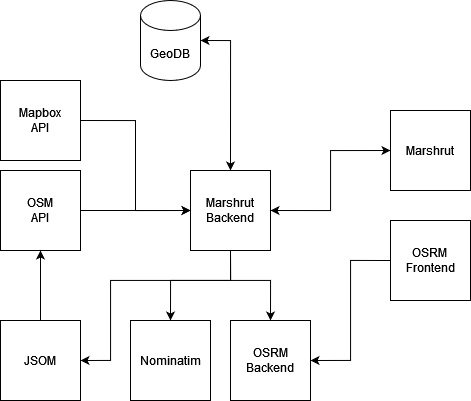
\includegraphics[width=0.5\textwidth]{images/SystemOverview.png}
  \caption{
  OSM Data Overview.
  }
  %for reference to this figure
  \label{figure:SystemOverview}
\end{figure*}

\section{Data Sources}

To create the historical pedestrian traffic/walking patterns, a solid Data-set is needed so the routing engine can be configured to be adapted to the influence of the walking patterns. 

Searching for a Data-set that is viable for further analysis was not an easy task. There is no publicly available data from the city itself. Also, local research institutions contacted during the research period have no such data available. Therefore the OSM (OpenStreetMap) Project and its Database of public traces came in handy. Their collection is publicly accessible to be extracted, verified, classified, and then used to create a historical pedestrian traffic pattern for the part of the city that was used to create the alternative route.

% Struggles from Hashemi to relate here too.
% Cite:
%
%However, GPS traces are stored in plain text formats with no attached metadata such as, transpor- tation mode, length, or speed. This not only makes managing large volumes of GPS traces inefficient but also restricts the scale and scope of algorithms for human mobility pattern detection. Open Street Map (OSM), founded in UK in 2004 with more than 1 million registered users (Wood, 2013), is the most prominent volunteered geographic information devoted to providing a free map of the world empha- sizing the road networks. Road networks are built upon GPS traces uploaded by registered users and can be edited or updated manually at any time. A description can be associated to a GPS trace while being uploaded but there are no additional required metadata or restrictions (https://www.open- streetmap.org/traces; OpenStreetMap, n.d.). This means the transportation mode of the GPS trace (e.g. walking, motoring, or boating) cannot be known in the database which in turn limits the data- base’s applications. Besides, they do not store additional metadata, such as average speed or total length of the GPS trace which can be automatically calculated. Such metadata not only facilitates analyzing, mining, and visualizing large volumes of GPS traces, but also paves the path for automatic applications of GPS traces. Examples of such applications are automatic road and pedestrian network construction (Hashemi, 2017b), recognizing POIs (Bhattacharya, Kulik, & Bailey, 2015), developing intelligent location-based services (Liu & Karimi, 2006), detecting individual (Song et al., 2010), or collective (Becker et al., 2013; Harder, Nes, Jensen, Reinau, & Weber, 2012) mobility patterns, and real-time event detection which is of great value to municipalities, police, and fire departments.
%
%

The OSM Database of public traces consists of over 11 billion uploaded GPS points around the globe. \footnote{\url{https://planet.openstreetmap.org/statistics/data_stats.html}}

As the study's focus is the City of Salzburg, an appropriate bbox (Bounding box) covering the inner city and most of its close-to-be districts was selected. 

The reason for overlapping with towns and places around Salzburg is the OSM Editing API. Getting as many traces as possible leading into the city makes a more accurate estimation of pedestrian traffic possible. As the API is only taking routes that lead through the bbox , given a more extensive sample area than necessary for the route proposal was taken into account. The bbox taken is seen in Figure \ref{figure:BoundingBox}.

%figure* stretches figure over both columns
\begin{figure*}[t]
  \centering
  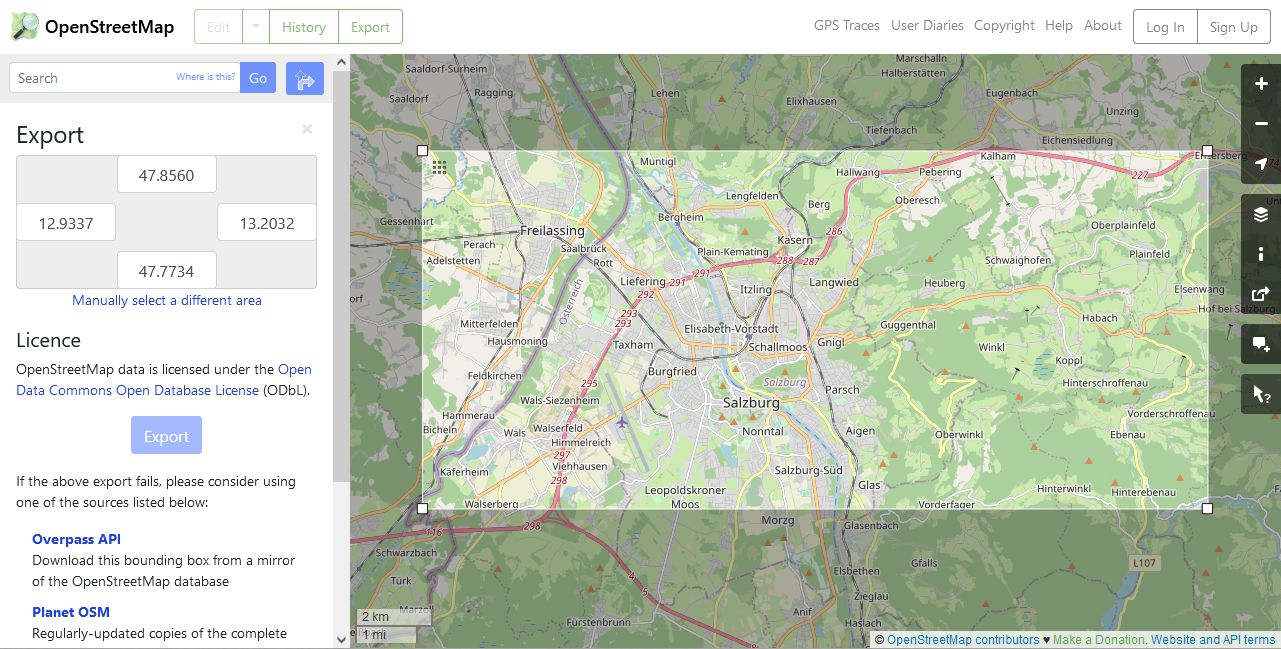
\includegraphics[width=0.9\textwidth]{images/BoundingBoxOSM.png}
  \caption{
  Bounding Box for extracted GPS trajectories.
  }
  %for reference to this figure
  \label{figure:BoundingBox}
\end{figure*}


\subsection{GPS Data}

Given the bbox of Salzburg and its surroundings, 595.000 Data-points were extracted using the OSM Editing API. \footnote{\url{https://wiki.openstreetmap.org/wiki/API_v0.6#GPS_traces}}

The OSM Editing API is a collection of APIs based on RESTful API principles. There are API calls to create, read, update, and delete the three fundamental elements that makeup OpenStreetMap's map data. They each return or expect the data for the elements in an XML format.
\autocite[]{wiki:xxx}

The Data-points are returned using GPX (GPS Exchange Format) a XML data format for GPS data \footnote{\url{https://www.topografix.com/GPX/1/1/#type_trksegType}}. Important to mention is that in violation of the GPX standard, for privacy reasons, all waypoints of non-trackable traces are randomized and delivered as one track segment. 

GPX (the GPS Exchange Format) is a light-weight XML data format for the interchange of GPS data (waypoints, routes, and tracks) between applications and Web services on the Internet. 

Important to mention is that This happens in violation of the GPX standard. 

To further work with the data points 

\subsection{Map Data}

%figure* stretches figure over both columns
\begin{figure*}[t]
  \centering
  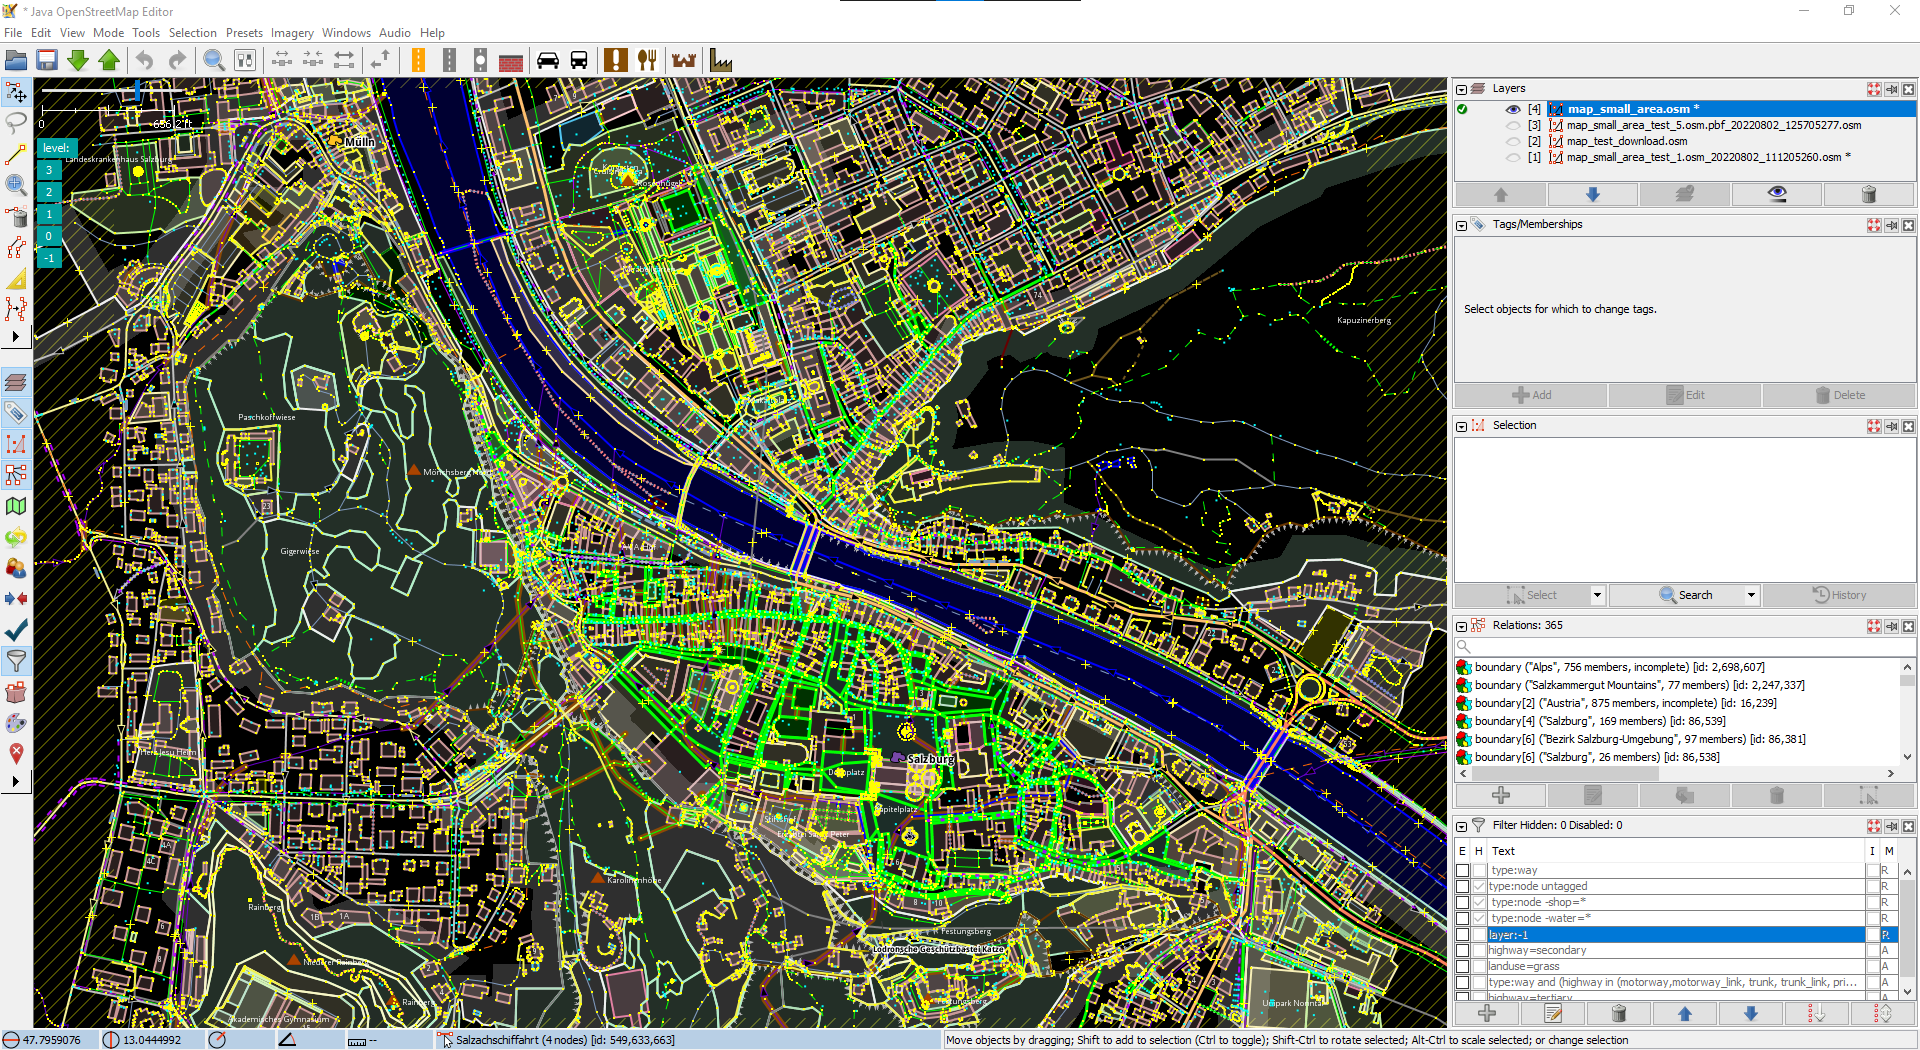
\includegraphics[width=0.9\textwidth]{images/DataOSM.png}
  \caption{
  OSM Data Overview.
  }
  %for reference to this figure
  \label{figure:MapData}
\end{figure*}

Same bbox

Consists of
- 28.158 nodes (2.929 incomplete)
- 19.427 ways (15.332 incomplete)
- 516 relations (197 incomplete)

- 333.831 nodes (7 incomplete)
- 43.604 ways (1.101 incomplete)
- 787 relations (422 incomplete)

%https://wiki.openstreetmap.org/wiki/JOSM_file_format
%https://wiki.openstreetmap.org/wiki/OSM_XML
%https://wiki.openstreetmap.org/wiki/PBF_Format

Further used for map-matching, geocoding & routing.

\section{Model & Implementation}

Provide implementation details such as the used software and our software architecture, highlight your own solutions to encountered difficulties. Describe relevant iterations of your implementation.

Before going deeper into the system architecture 
To go deeper into the system architecture 
Overview of the software basis used for the whole development: 
NodeJS, React,


Providing a route proposal starts further than analyzing geo-located trajectories. Precautious steps were needed in building the architecture to understand the data used for the newly suggested route. 

Therefore a Map Application was created to visualize the extracted and classified data, the routes used for the comparison, and the new suggested routes from the utilized routing engine. Said Map Application is a standalone React App using the Mapbox Plattform for map creation and route visualization. For working with React, Mapbox provides mapbox-gl-js, a javascript library that uses WebGL to render interactive maps from vector tiles and Mapbox styles.

%https://www.mapbox.com/
%https://docs.mapbox.com/mapbox-gl-js/guides/

For the map and route visualization to interact with the extracted geo trajectory data, a NodeJS backend was developed. The backend interacts with the OSM API and the established GeoDatabase, handling the trajectories' extraction, classification, and transformation.

With its geospatial data support, MongoDB was selected as the Geo-Database and stores the extracted Data-Set and the further classified data objects. Even though PostGIS is more mature and built on the Open Geospatial Consortium (OGC) standards, the uncertainty of incomplete data sets from the OSM project led to the decision to use the document-based solution.

To work with the OSM project and its map data, the JOSM (Java OpenStreetMap editor) was used to interact with the map layer as the basis for the route proposal. 
%https://josm.openstreetmap.de/

For the data extraction, a NodeJS backend interacting with the OSM API and the established GeoDatabase was created, handling the extraction, classification, and visualization of the trajectories and route suggestions.

Therefore a visualization of the City of Salzburg was built using the Mapbox Plattform. 
% https://docs.mapbox.com/mapbox-gl-js/guides/



% https://wiki.openstreetmap.org/wiki/Bounding_Box

\subsection{Database}

After the conversion the objects 
Working with Geodata there is 

MongoDB & Mongoose
% https://mongoosejs.com/docs/geojson.html
% https://www.mongodb.com/docs/manual/reference/geojson/

\subsection{Data Extraction}

Working with the OSM API

To retrieve the GPS track points 

https://api.openstreetmap.org/api/0.6/trackpoints?bbox=12.9337,47.7564,13.2032,47.8560&page=0

Get GPS Points: Get /api/0.6/trackpoints?bbox=left,bottom,right,top&page=pageNumber
Use this to retrieve the GPS track points that are inside a given bounding box (formatted in a GPX format).

Get GPS Points: Get /api/0.6/trackpoints?bbox=left,bottom,right,top&page=pageNumber


Use this to retrieve the GPS track points that are inside a given bounding box (formatted in a GPX format).

where:

left, bottom, right, and top are used the same way as they are in the command to retrieve nodes, ways, and relations.

pageNumber specifies which group of 5,000 points, or page, to return. Since the command does not return more than 5,000 points at a time, this parameter must be incremented—and the command sent again (using the same bounding box)—in order to retrieve all of the points for a bounding box that contains more than 5,000 points. When this parameter is 0 (zero), the command returns the first 5,000 points; when it is 1, the command returns points 5,001–10,000, etc.

% https://www.topografix.com/GPX/1/1/#type_trksegType

\begin{lstlisting}
<?xml version="1.0" encoding="UTF-8"?>
<gpx version="1.0" creator="OpenStreetMap.org" xmlns="http://www.topografix.com/GPX/1/0">
    <trk>
        <name>osmtrack_KUnrl0ZaKm.gpx</name>
        <desc>desc.</desc>
        <url>/user/exbrick/traces/3444105</url>
        <trkseg>
            <trkpt lat="47.8318200" lon="13.0567170">
                <time>2006-08-22T01:37:05Z</time>
            </trkpt>
            <trkpt lat="47.8325810" lon="13.0567800">
                <time>2006-08-22T01:37:20Z</time>
            </trkpt>
            <trkpt lat="47.8331180" lon="13.0569120">
                <time>2006-08-22T01:37:30Z</time>
            </trkpt>
            
\end{lstlisting}

\subsection{Data Prepocessing}

\subsubsection{Conversion}

As the objects returned from the API are in the GPX Format, a conversion step was needed to further work with the trajectories. As the MongoDB Database and the libraries used in the built Map Application are working with the GeoJSON standard \footnote{\url{https://datatracker.ietf.org/doc/html/rfc7946}}, a conversion step was necessary.

The conversion was achieved using the toGeoJSON tool \footnote{\url{https://github.com/mapbox/togeojson}} provided by Mapbox. After the first objects were converted, a significant number of them had attributes missing after the conversion. Therefore, the tool was adapted according to the GPX Formats' given attributes used by the OSM API.  

Attributes added: Properties

Using the tool togeojson provided by Mapbox the conversion was 

% https://github.com/mapbox/togeojson

\subsubsection{Outlier Removal}



\subsection{Map-Matching}

\subsubsection{OSRM}
\subsubsection{Mapbox}

OSRM & Mapbox



\autocite[]{Delling2012}

\subsection{Data Classification}

The Data Classifci

However, GPS traces are stored in plain text formats with no attached metadata such as, transportation mode, length, or speed. This not only makes managing large volumes of GPS traces inefficient but also restricts the scale and scope of algorithms for human mobility pattern detection

Road networks are built upon GPS traces uploaded by registered users and can be edited or updated manually at any time. A description can be associated to a GPS trace while being uploaded but there are no additional required metadata or restrictions

 This means the transportation mode of the GPS trace (e.g. walking, motoring, or boating) cannot be known in the database which in turn limits the data- base’s applications. Besides, they do not store additional metadata, such as average speed or total length of the GPS trace which can be automatically calculated. Such metadata not only facilitates analyzing, mining, and visualizing large volumes of GPS traces, but also paves the path for automatic applications of GPS traces.


\autocite[]{Zhang2012}

As the OSM GPS Traces are randomized and 

Count 533

3 Layers

Finding Routes Name / Description Car / Auto

NameCnt: 76
DescCnt: 8
Count: 397

Avg speed on total route

Avg speed using segmentation




TurfJS


osrm

Mapbox API


%However, GPS traces are stored in plain text formats with no attached metadata such as, transportation mode, length, or speed. This not only makes managing large volumes of GPS traces inefficient but also restricts the scale and scope of algorithms for human mobility pattern detection. Open Street Map (OSM), founded in UK in 2004 with more than 1 million registered users (Wood, 2013), is the most prominent volunteered geographic information devoted to providing a free map of the world emphasizing the road networks. Road networks are built upon GPS traces uploaded by registered users and can be edited or updated manually at any time. A description can be associated to a GPS trace while being uploaded but there are no additional required metadata or restrictions (https://www.open- streetmap.org/traces; OpenStreetMap, n.d.). This means the transportation mode of the GPS trace (e.g. walking, motoring, or boating) cannot be known in the database which in turn limits the data- base’s applications. Besides, they do not store additional metadata, such as average speed or total length of the GPS trace which can be automatically calculated. Such metadata not only facilitates analyzing, mining, and visualizing large volumes of GPS traces, but also paves the path for automatic applications of GPS traces. Examples of such applications are automatic road and pedestrian network construction (Hashemi, 2017b), recognizing POIs (Bhattacharya, Kulik, & Bailey, 2015), developing intelligent location-based services (Liu & Karimi, 2006), detecting individual (Song et al., 2010), or collective (Becker et al., 2013; Harder, Nes, Jensen, Reinau, & Weber, 2012) mobility patterns, and real-time event detection which is of great value to municipalities, police, and fire departments.



\subsection{Reverse Geo-coding}

nominatim



\subsection{Map Adaptations}

JOSM




\subsection{Routing}

Routing Engine

Profile adaption

\begin{lstlisting}
        smoothness_speeds = {
            excellent = walking_speed,
            bad = walking_speed * 0.5,

            one = walking_speed*0.01,
            two = walking_speed*0.02,

            three = walking_speed*0.001,
            four = walking_speed*0.004,
            
            five = walking_speed*0.005,
            six = walking_speed*0.006,
        }
\end{lstlisting}

\autocite[]{Delling2012}


\section{Evaluation}
%Describe your methodology. How did you evaluate your work? Why did you choose this methodology? Present results of your evaluation here.

To evaluate the research and to measure a possible increase in satisfaction of the route proposal a trail run of both routes was conducted.

\subsection{Methodology}

A qualitative trail run was conducted to measure a possible increase in satisfaction with the route proposal. In the trial run, a standard route was compared to the newly proposed route and measured using one survey. 

The survey was structured in three parts. Part number one used a quantitative method to determine the subjects demographics and general walking and route choosing behavior. Part number two measures the satisfaction of both routes. And part number three compares the routes within each other.

Finding out about the subjects' general walking and route choosing behavior should give a better understanding of the route satisfaction part results. Furthermore, it will give a relation to the increase or decrease in satisfaction.





Survey number one uses a quantitative method to determine the subjects' general travel behavior, while survey number two compares and measures satisfaction with a quantitative approach after the trial run.



Quantitative Surveys.




In present work, various research methods have been applied. They include a descriptive method (outlining different approaches to the term "actorness" and identifying the ways of measuring it), a historical method (following the historical development of the shared energy and environmental policies in the EU and their adaptation to the realities of the modern world), a comparative method (e.g., conferring the definitions of actorness and the level of actorness of the EU in energy and environmental spheres), statistical and quantitative (e.g., providing statistical data on the ecological goals and sustainable development, import of energy resources), analytical (e.g., assuming how the public opinion on the ecological situation contributes to the changing of the adopted energy policies), and process tracing method (e.g., identifying the causal mechanisms that link opportunity, presence, capability, performance, and effect, i.e., EU actorness).




\subsection{Survey}



\subsubsection{Demographics}

1. What is your age?
0-15 years
15-30 years
30-45 years
45+
 Prefer not to say

2. What gender do you feel you belong?
Female
Male
Prefer not to say

3. What is your highest educational qualification?
No compulsory education 
Compulsory school or secondary school (polytechnic school)
Apprenticeship 
Vocational middle school without Matura (e.g., 3-year HBLA/HLWM) 
General education or vocational higher school with Matura (e.g., Gymnasium, HTL, HAK, HLWM, HBLA) 
Bachelor's Degree
Master's Degree
Ph.D. or higher
Prefer not to say

4. What would you describe the area you’re living in as?
Urban
Rural

5. How long have you been living in Salzburg?
 ~1 year
 1-5 years
 5-10 years
10+ years

6. Do you drive a car?
Yes
No


\subsubsection{General Walking Behavior}

7. What are the purposes of your walk trips in general? (Choose a few)
Exercise/outdoor recreation
Grocery/food shopping
Personal business
Medical appointment
Entertainment
Dining at restaurants or bars
Commute to work
Other work-related travel
Other
No walking

8. How frequent do you take walking trips per month?
1 to 2 trips
3 to 6 trips
7 to 10 trips
11 to 19 trips
20 trips or more

9. How long are your walking trips in general?
5 to 10 minutes
10 to 20 minutes
20 to 40 minutes
40 to 60 minutes
Greater than 60

10. Do you take walk trips on vacation?
Yes
No


\subsubsection{Route Choosing Behavior}

11. How do you plan your route?
Physical map
Map Application (Google Maps, …)
Tour guide
Other, please specify: __________________

12. When do you plan your route?
Before the trip
On the spot

13. What are the main factors for your route planning? (Choose up to 3)
Travel Time
Distance
Least directional changes
Road Condition
Crowdedness
Many attractive places
Weather

14. When you are on vacation does your route planning change?
Yes
No

14.1 If yes, what factors do change?
Travel Time
Distance
Least directional changes
Road Condition
Crowdedness
Many attractive places
Weather

\subsubsection{Route A}


15. How was the travel time on the route? 
Unsatisfying



Satisfying

16. How crowded was the route?
Deserted



Very Crowded

17. How much you were satisfied by the route overall? 
Very unsatisfied



Very satisfied

18. What were the factors leading to this level of satisfaction?
Travel Time
Distance
Least directional changes
Road Condition
Crowdedness
Many attractive places
Weather

\subsubsection{Route B}

19. How was the travel time on the route? 
Unsatisfying



Satisfying

20. How crowded was the route?
Deserted



Very Crowded

21. How much you were satisfied by the route overall? 
Very unsatisfied



Very satisfied

22. What were the factors leading to this level of satisfaction?
Travel Time
Distance
Least directional changes
Road Condition
Crowdedness
Many attractive places
Weather

\subsubsection{Route Comparison}

23. Which of the two routes satisfied you more?
Route A
Route B

24. Which of the two routes was less crowded?
Route A
Route B

25. Would you take one of the routes if not given?
 Yes
 No

25.1 If yes, which one?
Route A
Route B


Part 1
Part 2
Part 3

\subsection{Trial run}

The trial run was executed with 25 people in the span of one weekend.

Weather day one

Weather day two

Weather day three

On each day runs were done during different times of the day reaching from 09:00 to 18:00. 


\subsection{Results}

\section{Discussion}
Discuss your results to answer your research question. Does your data support you hypotheses? Put your results into perspective by situating it in the research field/related work.

\section{Conclusion and Future Work}
Summarize your work, outline limitations and future work. 

% \section{Formatierung}
% \label{section:Formatting}

% Text mit beliebigen Sonderzeichen in UTF-8 ohne BOM \ldots
% ,
% \textbf{hervorgehobener Text},
% \texttt{void}\footnote{Fußnote 1},
% mathematische Formel im Text $\sum_{i=0}^n i^2$
% \ldots

% Referenz auf Unterabschnitt \ref{subsection:Coding} der Arbeit, automatisch richtig nummeriert.

% \textcite[]{Mulloni:2010} für einen einen Literaturverweis im laufenden Text.

% Literaturverweise sind essentiell für eine wissenschafliche Arbeit. \autocite[]{McConnell:2004:CCS:1096143}.

% Achtung: nur zitierte Literatur wird im Literaturverzeichnis
% angeführt.\footnote{Fußnote 2}


% Wir verwenden \LaTeX\footnote{ \url{http://en.wikibooks.org/wiki/LaTeX}} -- und das
% ist keine Quelle, sondern blos eine URL.

% \subsection{Figures machen was sie wollen}

% % h = try to place the figure Here
% % t = try to place the figure at the Top of a page
% % p = try to place this figure along with others on a separate Page
% % Note that LaTeX has a sophisticated ranking algorithm to place figures.
% % It is not always easy to accept LaTeX's placing but it is harder doing it
% % manually. Just let it go ;-)
% \begin{figure}[!ht]
% 	\centering
% 	\subfloat[Das Julia Fraktal]{
% 		\includegraphics[width=0.75\linewidth]{images/Julia-Fractal.png}
% 		%for reference of this subfigure only
% 		\label{subfigure:Julia-Fractal}
% 	}
% 	\qquad
% 	\subfloat[Noise für Tinteneffekte]{
% 		\includegraphics[width=0.75\linewidth]{images/Perlin-Coherent.png}
% 		%for reference of this subfigure only
% 		\label{subfigure:Perlin-Coherent}
% 	}
% 	\caption[
% 		Verschiedene Pixelgraphiken\newline
% 		% source url given in the table of figures
% 		\small\texttt{https://mediacube.at/wiki/}
% 	]{
% 		Verschiedene Pixelgraphiken
% 	}
% 	%for reference to all subfigures
% 	\label{figure:PixelImages}
% \end{figure}

% Unterstützte Pixelgraphikformate: PNG, JPEG, PDF.
% Angabe von height oder width meist wichtig.

% Referenz auf Abbildung \ref{figure:PixelImages} mit allen Teilbildern.
% Referenz auf Unterabbildung \ref{subfigure:Julia-Fractal}.

% %figure* stretches figure over both columns
% \begin{figure*}[t]
% 	\centering
% 	\includegraphics[width=0.9\textwidth]{images/KappaGamma.pdf}
% 	\caption{
% 		Vektorgraphik mit \LaTeX\ Beschriftung ($\kappa$, $\gamma$)
% 	}
% 	%for reference to this figure
% 	\label{figure:KappaGammaTau}
% \end{figure*}

% Referenz auf Abbildung \ref{figure:KappaGammaTau}.

% Bei Vektorgraphik mit \LaTeX\ Beschriftung keine Skalierung mit width oder height verwenden.

% Vektorgraphik mit \LaTeX\ Beschriftung kann etwa mit \texttt{ipe} erstellt werden.

% Unterstütztes Vektorgraphikformat: PDF. EPS muss konvertiert werden.


% \subsection{Unterabschnitt 2}
% %for references to this subsection
% \label{subsection:Coding}

% \begin{lstlisting}[
% 	label=listing:Main, %for reference to this listing
% 	float=h,
% 	caption=main.cpp,
% 	firstnumber=10
% ]
% int main(void) {
% 	while (true) {
% 	}
% 	return 0;
% }
% \end{lstlisting}

% Wie man in Listing \ref{listing:Main} in Zeile 10 sieht, kann man die Zeilennummern im Listing absichtlich setzen, hier z.B. auf 10. In Listing \ref{listing:closure} wurde davon nicht Gebrauch gemacht. In diesem Fall beginnt die Nummerierung bei 1.

% \begin{lstlisting}[
%     label=listing:closure,
% 	float=h,
% 	caption=Closure in Javascript,
% 	language=JavaScript
% ]
% function foo(x,y) {
%     let i = x;
%     return function(a) {
%         return i * 2;
%     }
% }
% \end{lstlisting}


% \subsubsection{Unterunterabschnitt i}

% Wörtliches Zitat:
% %select proper language if not in German
% \selectlanguage{english}
% \begin{quote}
% ``Erwin Unruh discovered that templates can be used to compute
% something at compile time. [...] The intriguing part of this exercise, however, was that the production of the prime numbers was performed by the compiler during the compilation process and not at run time.''

% \autocite[305]{Bosch2014}
% \end{quote}
% %select German again or the language that you were using before (note ngerman stands for New German)
% %\selectlanguage{ngerman}
% \selectthesislanguage


% \subsection{Unterabschnitt b}

% \begin{enumerate}
% 	\item Punkt 1
% 	\begin{enumerate}
% 		\item Unterpunkt 1
% 		\item Unterpunkt 2
% 	\end{enumerate}
% 	\item Punkt 2
% \end{enumerate}

% \begin{itemize}
% 	\item Punkt 1
% 	\begin{itemize}
% 		\item Unterpunkt 1
% 		\item Unterpunkt 2
% 	\end{itemize}
% 	\item Punkt 2
% \end{itemize}


% \subsection{Unterabschnitt c}

% \begin{table}[ht]
% 	\centering
% 	\begin{tabular}{r|rrr}
% 		    & $i$ & $j$ & $k$ \\ \hline
% 		$i$ &$-1$ & $k$ &$-j$ \\
% 		$j$ &$-k$ &$-1$ & $i$ \\
% 		$k$ & $j$ &$-i$ &$-1$
% 	\end{tabular}
% 	\caption{
% 		Multiplikationstabelle für Quaternionen
% 	}
% 	\label{table:Quaternions}
% \end{table}

% Referenz auf Tabelle \ref{table:Quaternions}.

% \section{Abschnitt 2}
% \label{section:MathematicalStuff}

% Sei $f(x)$ eine stetige Funktion, so ist die \textbf{Fourier Transformierte}
% $F(\omega)$ wie folgt definiert:
% \begin{equation}
% \label{equation:FourierDefinition}
% 	F(\omega) = \int_{-\infty}^{\infty} f(x) e^{-i\omega t} dt
% \end{equation}

% Referenz auf mathematische Gleichung (\ref{equation:FourierDefinition}).

% Unnummerierte Gleichung:
% \begin{equation*}
% 	e^{i\varphi} = \cos\varphi + i \sin\varphi
% \end{equation*}
% %you may also use \[ \] instead of \begin{equation*} and \end{equation*}

% Gleichungssystem:
% \begin{eqnarray}
% 	g(x) = f(x - x_0) & \Leftrightarrow &
% 		G(\omega) = F(\omega) e^{-i\omega x_0} \\
% 	g(x) = f(x) e^{i\omega_0 x} & \Leftrightarrow &
% 		G(\omega) = F(\omega - \omega_0)
% \end{eqnarray}
